% Graphic for TeX using PGF
% Title: /home/gabs48/mit/thesis/graphic/calib_arch.dia
% Creator: Dia v0.97.2
% CreationDate: Fri Oct 10 14:03:20 2014
% For: gabs48
% \usepackage{tikz}
% The following commands are not supported in PSTricks at present
% We define them conditionally, so when they are implemented,
% this pgf file will use them.
\ifx\du\undefined
  \newlength{\du}
\fi
\setlength{\du}{15\unitlength}
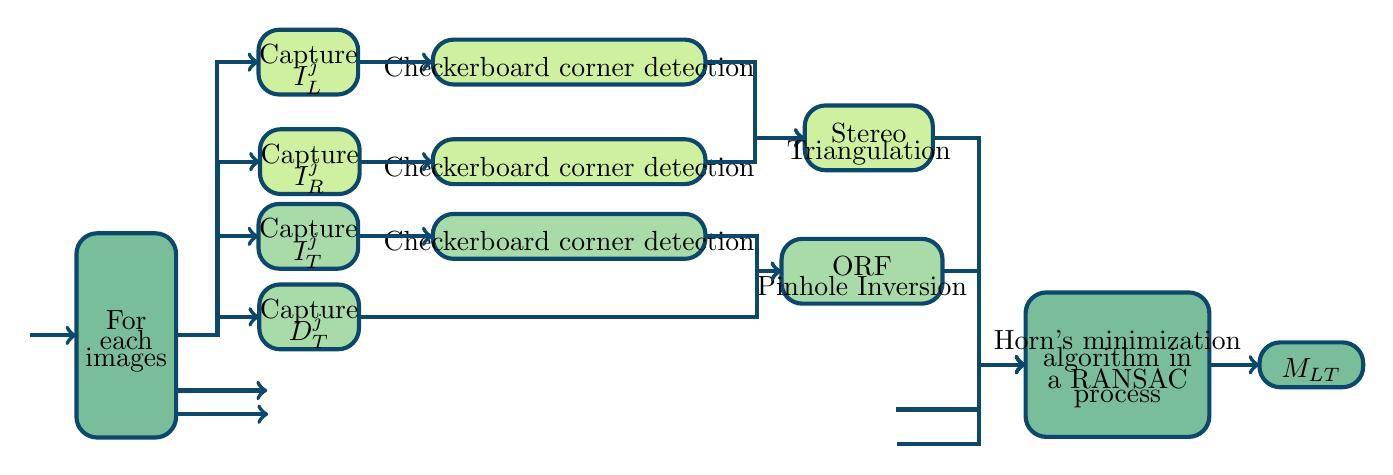
\begin{tikzpicture}
\pgftransformxscale{0.600000}
\pgftransformyscale{-0.600000}
\definecolor{dialinecolor}{rgb}{0.000000, 0.000000, 0.000000}
\pgfsetstrokecolor{dialinecolor}
\definecolor{dialinecolor}{rgb}{1.000000, 1.000000, 1.000000}
\pgfsetfillcolor{dialinecolor}
\pgfsetlinewidth{0.100000\du}
\pgfsetdash{}{0pt}
{\pgfsetcornersarced{\pgfpoint{0.500000\du}{0.500000\du}}\definecolor{dialinecolor}{rgb}{0.811765, 0.941176, 0.619608}
\pgfsetfillcolor{dialinecolor}
\fill (15.000000\du,11.000000\du)--(15.000000\du,12.800000\du)--(25.947500\du,12.800000\du)--(25.947500\du,11.000000\du)--cycle;
}{\pgfsetcornersarced{\pgfpoint{0.500000\du}{0.500000\du}}\definecolor{dialinecolor}{rgb}{0.043137, 0.282353, 0.419608}
\pgfsetstrokecolor{dialinecolor}
\draw (15.000000\du,11.000000\du)--(15.000000\du,12.800000\du)--(25.947500\du,12.800000\du)--(25.947500\du,11.000000\du)--cycle;
}% setfont left to latex
\definecolor{dialinecolor}{rgb}{0.043137, 0.282353, 0.419608}
\pgfsetstrokecolor{dialinecolor}
\node at (20.473750\du,12.095000\du){Checkerboard corner detection};
\pgfsetlinewidth{0.100000\du}
\pgfsetdash{}{0pt}
{\pgfsetcornersarced{\pgfpoint{0.500000\du}{0.500000\du}}\definecolor{dialinecolor}{rgb}{0.811765, 0.941176, 0.619608}
\pgfsetfillcolor{dialinecolor}
\fill (15.000000\du,15.000000\du)--(15.000000\du,16.800000\du)--(25.947500\du,16.800000\du)--(25.947500\du,15.000000\du)--cycle;
}{\pgfsetcornersarced{\pgfpoint{0.500000\du}{0.500000\du}}\definecolor{dialinecolor}{rgb}{0.043137, 0.282353, 0.419608}
\pgfsetstrokecolor{dialinecolor}
\draw (15.000000\du,15.000000\du)--(15.000000\du,16.800000\du)--(25.947500\du,16.800000\du)--(25.947500\du,15.000000\du)--cycle;
}% setfont left to latex
\definecolor{dialinecolor}{rgb}{0.043137, 0.282353, 0.419608}
\pgfsetstrokecolor{dialinecolor}
\node at (20.473750\du,16.095000\du){Checkerboard corner detection};
\pgfsetlinewidth{0.100000\du}
\pgfsetdash{}{0pt}
{\pgfsetcornersarced{\pgfpoint{0.500000\du}{0.500000\du}}\definecolor{dialinecolor}{rgb}{0.658824, 0.858824, 0.658824}
\pgfsetfillcolor{dialinecolor}
\fill (15.000000\du,18.000000\du)--(15.000000\du,19.800000\du)--(25.947500\du,19.800000\du)--(25.947500\du,18.000000\du)--cycle;
}{\pgfsetcornersarced{\pgfpoint{0.500000\du}{0.500000\du}}\definecolor{dialinecolor}{rgb}{0.043137, 0.282353, 0.419608}
\pgfsetstrokecolor{dialinecolor}
\draw (15.000000\du,18.000000\du)--(15.000000\du,19.800000\du)--(25.947500\du,19.800000\du)--(25.947500\du,18.000000\du)--cycle;
}% setfont left to latex
\definecolor{dialinecolor}{rgb}{0.043137, 0.282353, 0.419608}
\pgfsetstrokecolor{dialinecolor}
\node at (20.473750\du,19.095000\du){Checkerboard corner detection};
\pgfsetlinewidth{0.100000\du}
\pgfsetdash{}{0pt}
{\pgfsetcornersarced{\pgfpoint{0.500000\du}{0.500000\du}}\definecolor{dialinecolor}{rgb}{0.658824, 0.858824, 0.658824}
\pgfsetfillcolor{dialinecolor}
\fill (29.000000\du,19.000000\du)--(29.000000\du,21.600000\du)--(35.465000\du,21.600000\du)--(35.465000\du,19.000000\du)--cycle;
}{\pgfsetcornersarced{\pgfpoint{0.500000\du}{0.500000\du}}\definecolor{dialinecolor}{rgb}{0.043137, 0.282353, 0.419608}
\pgfsetstrokecolor{dialinecolor}
\draw (29.000000\du,19.000000\du)--(29.000000\du,21.600000\du)--(35.465000\du,21.600000\du)--(35.465000\du,19.000000\du)--cycle;
}% setfont left to latex
\definecolor{dialinecolor}{rgb}{0.043137, 0.282353, 0.419608}
\pgfsetstrokecolor{dialinecolor}
\node at (32.232500\du,20.095000\du){ORF};
% setfont left to latex
\definecolor{dialinecolor}{rgb}{0.043137, 0.282353, 0.419608}
\pgfsetstrokecolor{dialinecolor}
\node at (32.232500\du,20.895000\du){Pinhole Inversion};
\pgfsetlinewidth{0.100000\du}
\pgfsetbuttcap
\pgfsetdash{}{0pt}
{
\definecolor{dialinecolor}{rgb}{0.043137, 0.282353, 0.419608}
\pgfsetfillcolor{dialinecolor}
% was here!!!
\pgfsetarrowsend{to}
\definecolor{dialinecolor}{rgb}{0.043137, 0.282353, 0.419608}
\pgfsetstrokecolor{dialinecolor}
\draw (25.947500\du,11.900000\du)--(27.941049\du,11.900000\du)--(27.941049\du,14.944005\du)--(29.934598\du,14.944005\du);
}
% setfont left to latex
\pgfsetlinewidth{0.100000\du}
\pgfsetbuttcap
\pgfsetdash{}{0pt}
{
\definecolor{dialinecolor}{rgb}{0.043137, 0.282353, 0.419608}
\pgfsetfillcolor{dialinecolor}
% was here!!!
\pgfsetarrowsend{to}
\definecolor{dialinecolor}{rgb}{0.043137, 0.282353, 0.419608}
\pgfsetstrokecolor{dialinecolor}
\draw (25.947500\du,15.900000\du)--(27.941049\du,15.900000\du)--(27.941049\du,14.944005\du)--(29.934598\du,14.944005\du);
}
% setfont left to latex
\pgfsetlinewidth{0.100000\du}
\pgfsetbuttcap
\pgfsetdash{}{0pt}
{
\definecolor{dialinecolor}{rgb}{0.043137, 0.282353, 0.419608}
\pgfsetfillcolor{dialinecolor}
% was here!!!
\pgfsetarrowsend{to}
\definecolor{dialinecolor}{rgb}{0.043137, 0.282353, 0.419608}
\pgfsetstrokecolor{dialinecolor}
\draw (25.997624\du,18.900000\du)--(28.000000\du,18.900000\du)--(28.000000\du,20.300000\du)--(29.000000\du,20.300000\du);
}
% setfont left to latex
\pgfsetlinewidth{0.100000\du}
\pgfsetbuttcap
\pgfsetdash{}{0pt}
{
\definecolor{dialinecolor}{rgb}{0.043137, 0.282353, 0.419608}
\pgfsetfillcolor{dialinecolor}
% was here!!!
\pgfsetarrowsend{to}
\definecolor{dialinecolor}{rgb}{0.043137, 0.282353, 0.419608}
\pgfsetstrokecolor{dialinecolor}
\draw (12.001417\du,11.903914\du)--(13.500708\du,11.903914\du)--(13.500708\du,11.900000\du)--(15.000000\du,11.900000\du);
}
% setfont left to latex
\pgfsetlinewidth{0.100000\du}
\pgfsetbuttcap
\pgfsetdash{}{0pt}
{
\definecolor{dialinecolor}{rgb}{0.043137, 0.282353, 0.419608}
\pgfsetfillcolor{dialinecolor}
% was here!!!
\pgfsetarrowsend{to}
\definecolor{dialinecolor}{rgb}{0.043137, 0.282353, 0.419608}
\pgfsetstrokecolor{dialinecolor}
\draw (12.060496\du,15.898733\du)--(13.525000\du,15.898733\du)--(13.525000\du,15.900000\du)--(15.000000\du,15.900000\du);
}
% setfont left to latex
\pgfsetlinewidth{0.100000\du}
\pgfsetbuttcap
\pgfsetdash{}{0pt}
{
\definecolor{dialinecolor}{rgb}{0.043137, 0.282353, 0.419608}
\pgfsetfillcolor{dialinecolor}
% was here!!!
\pgfsetarrowsend{to}
\definecolor{dialinecolor}{rgb}{0.043137, 0.282353, 0.419608}
\pgfsetstrokecolor{dialinecolor}
\draw (12.001482\du,18.897713\du)--(13.500741\du,18.897713\du)--(13.500741\du,18.900000\du)--(15.000000\du,18.900000\du);
}
% setfont left to latex
\pgfsetlinewidth{0.100000\du}
\pgfsetbuttcap
\pgfsetdash{}{0pt}
{
\definecolor{dialinecolor}{rgb}{0.043137, 0.282353, 0.419608}
\pgfsetfillcolor{dialinecolor}
% was here!!!
\pgfsetarrowsend{to}
\definecolor{dialinecolor}{rgb}{0.043137, 0.282353, 0.419608}
\pgfsetstrokecolor{dialinecolor}
\draw (12.033259\du,22.131456\du)--(28.000000\du,22.131456\du)--(28.000000\du,20.300000\du)--(29.000000\du,20.300000\du);
}
% setfont left to latex
\pgfsetlinewidth{0.100000\du}
\pgfsetdash{}{0pt}
{\pgfsetcornersarced{\pgfpoint{0.500000\du}{0.500000\du}}\definecolor{dialinecolor}{rgb}{0.474510, 0.741176, 0.603922}
\pgfsetfillcolor{dialinecolor}
\fill (38.800000\du,21.150000\du)--(38.800000\du,26.950000\du)--(46.177500\du,26.950000\du)--(46.177500\du,21.150000\du)--cycle;
}{\pgfsetcornersarced{\pgfpoint{0.500000\du}{0.500000\du}}\definecolor{dialinecolor}{rgb}{0.043137, 0.282353, 0.419608}
\pgfsetstrokecolor{dialinecolor}
\draw (38.800000\du,21.150000\du)--(38.800000\du,26.950000\du)--(46.177500\du,26.950000\du)--(46.177500\du,21.150000\du)--cycle;
}% setfont left to latex
\definecolor{dialinecolor}{rgb}{0.043137, 0.282353, 0.419608}
\pgfsetstrokecolor{dialinecolor}
\node at (42.488750\du,22.245000\du){};
% setfont left to latex
\definecolor{dialinecolor}{rgb}{0.043137, 0.282353, 0.419608}
\pgfsetstrokecolor{dialinecolor}
\node at (42.488750\du,23.045000\du){Horn's minimization};
% setfont left to latex
\definecolor{dialinecolor}{rgb}{0.043137, 0.282353, 0.419608}
\pgfsetstrokecolor{dialinecolor}
\node at (42.488750\du,23.845000\du){algorithm in};
% setfont left to latex
\definecolor{dialinecolor}{rgb}{0.043137, 0.282353, 0.419608}
\pgfsetstrokecolor{dialinecolor}
\node at (42.488750\du,24.645000\du){a RANSAC};
% setfont left to latex
\definecolor{dialinecolor}{rgb}{0.043137, 0.282353, 0.419608}
\pgfsetstrokecolor{dialinecolor}
\node at (42.488750\du,25.445000\du){process};
% setfont left to latex
\definecolor{dialinecolor}{rgb}{0.043137, 0.282353, 0.419608}
\pgfsetstrokecolor{dialinecolor}
\node at (42.488750\du,26.245000\du){};
\pgfsetlinewidth{0.100000\du}
\pgfsetbuttcap
\pgfsetdash{}{0pt}
{
\definecolor{dialinecolor}{rgb}{0.043137, 0.282353, 0.419608}
\pgfsetfillcolor{dialinecolor}
% was here!!!
\pgfsetarrowsend{to}
\definecolor{dialinecolor}{rgb}{0.043137, 0.282353, 0.419608}
\pgfsetstrokecolor{dialinecolor}
\draw (35.465000\du,20.300000\du)--(36.917982\du,20.300000\du)--(36.917982\du,24.050000\du)--(38.800000\du,24.050000\du);
}
% setfont left to latex
\pgfsetlinewidth{0.100000\du}
\pgfsetbuttcap
\pgfsetdash{}{0pt}
{
\definecolor{dialinecolor}{rgb}{0.043137, 0.282353, 0.419608}
\pgfsetfillcolor{dialinecolor}
% was here!!!
\pgfsetarrowsend{to}
\definecolor{dialinecolor}{rgb}{0.043137, 0.282353, 0.419608}
\pgfsetstrokecolor{dialinecolor}
\draw (35.074598\du,14.944005\du)--(36.937299\du,14.944005\du)--(36.937299\du,24.050000\du)--(38.800000\du,24.050000\du);
}
% setfont left to latex
\pgfsetlinewidth{0.100000\du}
\pgfsetbuttcap
\pgfsetdash{}{0pt}
{
\definecolor{dialinecolor}{rgb}{0.043137, 0.282353, 0.419608}
\pgfsetfillcolor{dialinecolor}
% was here!!!
\pgfsetarrowsend{to}
\definecolor{dialinecolor}{rgb}{0.043137, 0.282353, 0.419608}
\pgfsetstrokecolor{dialinecolor}
\draw (33.600000\du,25.850000\du)--(36.917982\du,25.850000\du)--(36.917982\du,24.050000\du)--(38.800000\du,24.050000\du);
}
% setfont left to latex
\pgfsetlinewidth{0.100000\du}
\pgfsetbuttcap
\pgfsetdash{}{0pt}
{
\definecolor{dialinecolor}{rgb}{0.043137, 0.282353, 0.419608}
\pgfsetfillcolor{dialinecolor}
% was here!!!
\pgfsetarrowsend{to}
\definecolor{dialinecolor}{rgb}{0.043137, 0.282353, 0.419608}
\pgfsetstrokecolor{dialinecolor}
\draw (33.650000\du,27.250000\du)--(36.917982\du,27.250000\du)--(36.917982\du,24.050000\du)--(38.800000\du,24.050000\du);
}
% setfont left to latex
\pgfsetlinewidth{0.100000\du}
\pgfsetbuttcap
\pgfsetdash{}{0pt}
{
\definecolor{dialinecolor}{rgb}{0.043137, 0.282353, 0.419608}
\pgfsetfillcolor{dialinecolor}
% was here!!!
\pgfsetarrowsend{to}
\definecolor{dialinecolor}{rgb}{0.043137, 0.282353, 0.419608}
\pgfsetstrokecolor{dialinecolor}
\draw (46.177500\du,24.050000\du)--(47.184333\du,24.050000\du)--(47.184333\du,24.056152\du)--(48.191166\du,24.056152\du);
}
% setfont left to latex
\pgfsetlinewidth{0.100000\du}
\pgfsetbuttcap
\pgfsetdash{}{0pt}
{
\definecolor{dialinecolor}{rgb}{0.043137, 0.282353, 0.419608}
\pgfsetfillcolor{dialinecolor}
% was here!!!
\pgfsetarrowsend{to}
\definecolor{dialinecolor}{rgb}{0.043137, 0.282353, 0.419608}
\pgfsetstrokecolor{dialinecolor}
\draw (4.692174\du,22.875052\du)--(6.346795\du,22.875052\du)--(6.346795\du,11.903914\du)--(8.001417\du,11.903914\du);
}
% setfont left to latex
\pgfsetlinewidth{0.100000\du}
\pgfsetbuttcap
\pgfsetdash{}{0pt}
{
\definecolor{dialinecolor}{rgb}{0.043137, 0.282353, 0.419608}
\pgfsetfillcolor{dialinecolor}
% was here!!!
\pgfsetarrowsend{to}
\definecolor{dialinecolor}{rgb}{0.043137, 0.282353, 0.419608}
\pgfsetstrokecolor{dialinecolor}
\draw (4.692174\du,22.875052\du)--(6.354436\du,22.875052\du)--(6.354436\du,15.898733\du)--(8.060496\du,15.898733\du);
}
% setfont left to latex
\pgfsetlinewidth{0.100000\du}
\pgfsetbuttcap
\pgfsetdash{}{0pt}
{
\definecolor{dialinecolor}{rgb}{0.043137, 0.282353, 0.419608}
\pgfsetfillcolor{dialinecolor}
% was here!!!
\pgfsetarrowsend{to}
\definecolor{dialinecolor}{rgb}{0.043137, 0.282353, 0.419608}
\pgfsetstrokecolor{dialinecolor}
\draw (4.692174\du,22.875052\du)--(6.346828\du,22.875052\du)--(6.346828\du,18.897713\du)--(8.001482\du,18.897713\du);
}
% setfont left to latex
\pgfsetlinewidth{0.100000\du}
\pgfsetbuttcap
\pgfsetdash{}{0pt}
{
\definecolor{dialinecolor}{rgb}{0.043137, 0.282353, 0.419608}
\pgfsetfillcolor{dialinecolor}
% was here!!!
\pgfsetarrowsend{to}
\definecolor{dialinecolor}{rgb}{0.043137, 0.282353, 0.419608}
\pgfsetstrokecolor{dialinecolor}
\draw (4.692174\du,22.875052\du)--(6.354436\du,22.875052\du)--(6.354436\du,22.131456\du)--(8.033259\du,22.131456\du);
}
% setfont left to latex
\pgfsetlinewidth{0.100000\du}
\pgfsetbuttcap
\pgfsetdash{}{0pt}
{
\definecolor{dialinecolor}{rgb}{0.043137, 0.282353, 0.419608}
\pgfsetfillcolor{dialinecolor}
% was here!!!
\pgfsetarrowsend{to}
\definecolor{dialinecolor}{rgb}{0.043137, 0.282353, 0.419608}
\pgfsetstrokecolor{dialinecolor}
\draw (4.695407\du,25.085925\du)--(6.523887\du,25.085925\du)--(6.523887\du,25.086641\du)--(8.352366\du,25.086641\du);
}
% setfont left to latex
\pgfsetlinewidth{0.100000\du}
\pgfsetbuttcap
\pgfsetdash{}{0pt}
{
\definecolor{dialinecolor}{rgb}{0.043137, 0.282353, 0.419608}
\pgfsetfillcolor{dialinecolor}
% was here!!!
\pgfsetarrowsend{to}
\definecolor{dialinecolor}{rgb}{0.043137, 0.282353, 0.419608}
\pgfsetstrokecolor{dialinecolor}
\draw (4.650000\du,26.038761\du)--(6.521277\du,26.038761\du)--(6.521277\du,26.038729\du)--(8.392555\du,26.038729\du);
}
% setfont left to latex
% setfont left to latex
\definecolor{dialinecolor}{rgb}{0.043137, 0.282353, 0.419608}
\pgfsetstrokecolor{dialinecolor}
\node[anchor=west] at (2.620301\du,20.636790\du){};
\pgfsetlinewidth{0.100000\du}
\pgfsetbuttcap
\pgfsetdash{}{0pt}
{
\definecolor{dialinecolor}{rgb}{0.043137, 0.282353, 0.419608}
\pgfsetfillcolor{dialinecolor}
% was here!!!
\pgfsetarrowsend{to}
\definecolor{dialinecolor}{rgb}{0.043137, 0.282353, 0.419608}
\pgfsetstrokecolor{dialinecolor}
\draw (-1.183208\du,22.861674\du)--(-0.149038\du,22.861674\du)--(-0.149038\du,22.875052\du)--(0.692174\du,22.875052\du);
}
% setfont left to latex
\pgfsetlinewidth{0.100000\du}
\pgfsetdash{}{0pt}
{\pgfsetcornersarced{\pgfpoint{0.500000\du}{0.500000\du}}\definecolor{dialinecolor}{rgb}{0.474510, 0.741176, 0.603922}
\pgfsetfillcolor{dialinecolor}
\fill (0.692174\du,18.775052\du)--(0.692174\du,26.975052\du)--(4.692174\du,26.975052\du)--(4.692174\du,18.775052\du)--cycle;
}{\pgfsetcornersarced{\pgfpoint{0.500000\du}{0.500000\du}}\definecolor{dialinecolor}{rgb}{0.043137, 0.282353, 0.419608}
\pgfsetstrokecolor{dialinecolor}
\draw (0.692174\du,18.775052\du)--(0.692174\du,26.975052\du)--(4.692174\du,26.975052\du)--(4.692174\du,18.775052\du)--cycle;
}% setfont left to latex
\definecolor{dialinecolor}{rgb}{0.043137, 0.282353, 0.419608}
\pgfsetstrokecolor{dialinecolor}
\node at (2.692174\du,19.870052\du){};
% setfont left to latex
\definecolor{dialinecolor}{rgb}{0.043137, 0.282353, 0.419608}
\pgfsetstrokecolor{dialinecolor}
\node at (2.692174\du,20.670052\du){};
% setfont left to latex
\definecolor{dialinecolor}{rgb}{0.043137, 0.282353, 0.419608}
\pgfsetstrokecolor{dialinecolor}
\node at (2.692174\du,21.470052\du){};
% setfont left to latex
\definecolor{dialinecolor}{rgb}{0.043137, 0.282353, 0.419608}
\pgfsetstrokecolor{dialinecolor}
\node at (2.692174\du,22.270052\du){For};
% setfont left to latex
\definecolor{dialinecolor}{rgb}{0.043137, 0.282353, 0.419608}
\pgfsetstrokecolor{dialinecolor}
\node at (2.692174\du,23.070052\du){each};
% setfont left to latex
\definecolor{dialinecolor}{rgb}{0.043137, 0.282353, 0.419608}
\pgfsetstrokecolor{dialinecolor}
\node at (2.692174\du,23.870052\du){images};
% setfont left to latex
\definecolor{dialinecolor}{rgb}{0.043137, 0.282353, 0.419608}
\pgfsetstrokecolor{dialinecolor}
\node at (2.692174\du,24.670052\du){};
% setfont left to latex
\definecolor{dialinecolor}{rgb}{0.043137, 0.282353, 0.419608}
\pgfsetstrokecolor{dialinecolor}
\node at (2.692174\du,25.470052\du){};
% setfont left to latex
\definecolor{dialinecolor}{rgb}{0.043137, 0.282353, 0.419608}
\pgfsetstrokecolor{dialinecolor}
\node at (2.692174\du,26.270052\du){};
\pgfsetlinewidth{0.100000\du}
\pgfsetdash{}{0pt}
{\pgfsetcornersarced{\pgfpoint{0.500000\du}{0.500000\du}}\definecolor{dialinecolor}{rgb}{0.811765, 0.941176, 0.619608}
\pgfsetfillcolor{dialinecolor}
\fill (29.934598\du,13.644005\du)--(29.934598\du,16.244005\du)--(35.074598\du,16.244005\du)--(35.074598\du,13.644005\du)--cycle;
}{\pgfsetcornersarced{\pgfpoint{0.500000\du}{0.500000\du}}\definecolor{dialinecolor}{rgb}{0.043137, 0.282353, 0.419608}
\pgfsetstrokecolor{dialinecolor}
\draw (29.934598\du,13.644005\du)--(29.934598\du,16.244005\du)--(35.074598\du,16.244005\du)--(35.074598\du,13.644005\du)--cycle;
}% setfont left to latex
\definecolor{dialinecolor}{rgb}{0.043137, 0.282353, 0.419608}
\pgfsetstrokecolor{dialinecolor}
\node at (32.504598\du,14.739005\du){Stereo};
% setfont left to latex
\definecolor{dialinecolor}{rgb}{0.043137, 0.282353, 0.419608}
\pgfsetstrokecolor{dialinecolor}
\node at (32.504598\du,15.539005\du){Triangulation};
\pgfsetlinewidth{0.100000\du}
\pgfsetdash{}{0pt}
{\pgfsetcornersarced{\pgfpoint{0.500000\du}{0.500000\du}}\definecolor{dialinecolor}{rgb}{0.811765, 0.941176, 0.619608}
\pgfsetfillcolor{dialinecolor}
\fill (8.001417\du,10.603914\du)--(8.001417\du,13.203914\du)--(12.001417\du,13.203914\du)--(12.001417\du,10.603914\du)--cycle;
}{\pgfsetcornersarced{\pgfpoint{0.500000\du}{0.500000\du}}\definecolor{dialinecolor}{rgb}{0.043137, 0.282353, 0.419608}
\pgfsetstrokecolor{dialinecolor}
\draw (8.001417\du,10.603914\du)--(8.001417\du,13.203914\du)--(12.001417\du,13.203914\du)--(12.001417\du,10.603914\du)--cycle;
}% setfont left to latex
\definecolor{dialinecolor}{rgb}{0.043137, 0.282353, 0.419608}
\pgfsetstrokecolor{dialinecolor}
\node at (10.001417\du,11.698914\du){Capture};
% setfont left to latex
\definecolor{dialinecolor}{rgb}{0.043137, 0.282353, 0.419608}
\pgfsetstrokecolor{dialinecolor}
\node at (10.001417\du,12.498914\du){$I_L^j$};
\pgfsetlinewidth{0.100000\du}
\pgfsetdash{}{0pt}
{\pgfsetcornersarced{\pgfpoint{0.500000\du}{0.500000\du}}\definecolor{dialinecolor}{rgb}{0.811765, 0.941176, 0.619608}
\pgfsetfillcolor{dialinecolor}
\fill (8.060496\du,14.598733\du)--(8.060496\du,17.198733\du)--(12.060496\du,17.198733\du)--(12.060496\du,14.598733\du)--cycle;
}{\pgfsetcornersarced{\pgfpoint{0.500000\du}{0.500000\du}}\definecolor{dialinecolor}{rgb}{0.043137, 0.282353, 0.419608}
\pgfsetstrokecolor{dialinecolor}
\draw (8.060496\du,14.598733\du)--(8.060496\du,17.198733\du)--(12.060496\du,17.198733\du)--(12.060496\du,14.598733\du)--cycle;
}% setfont left to latex
\definecolor{dialinecolor}{rgb}{0.043137, 0.282353, 0.419608}
\pgfsetstrokecolor{dialinecolor}
\node at (10.060496\du,15.693733\du){Capture};
% setfont left to latex
\definecolor{dialinecolor}{rgb}{0.043137, 0.282353, 0.419608}
\pgfsetstrokecolor{dialinecolor}
\node at (10.060496\du,16.493733\du){$I_R^j$};
\pgfsetlinewidth{0.100000\du}
\pgfsetdash{}{0pt}
{\pgfsetcornersarced{\pgfpoint{0.500000\du}{0.500000\du}}\definecolor{dialinecolor}{rgb}{0.658824, 0.858824, 0.658824}
\pgfsetfillcolor{dialinecolor}
\fill (8.001482\du,17.597713\du)--(8.001482\du,20.197713\du)--(12.001482\du,20.197713\du)--(12.001482\du,17.597713\du)--cycle;
}{\pgfsetcornersarced{\pgfpoint{0.500000\du}{0.500000\du}}\definecolor{dialinecolor}{rgb}{0.043137, 0.282353, 0.419608}
\pgfsetstrokecolor{dialinecolor}
\draw (8.001482\du,17.597713\du)--(8.001482\du,20.197713\du)--(12.001482\du,20.197713\du)--(12.001482\du,17.597713\du)--cycle;
}% setfont left to latex
\definecolor{dialinecolor}{rgb}{0.043137, 0.282353, 0.419608}
\pgfsetstrokecolor{dialinecolor}
\node at (10.001482\du,18.692713\du){Capture};
% setfont left to latex
\definecolor{dialinecolor}{rgb}{0.043137, 0.282353, 0.419608}
\pgfsetstrokecolor{dialinecolor}
\node at (10.001482\du,19.492713\du){$I_T^j$};
\pgfsetlinewidth{0.100000\du}
\pgfsetdash{}{0pt}
{\pgfsetcornersarced{\pgfpoint{0.500000\du}{0.500000\du}}\definecolor{dialinecolor}{rgb}{0.658824, 0.858824, 0.658824}
\pgfsetfillcolor{dialinecolor}
\fill (8.033259\du,20.831456\du)--(8.033259\du,23.431456\du)--(12.033259\du,23.431456\du)--(12.033259\du,20.831456\du)--cycle;
}{\pgfsetcornersarced{\pgfpoint{0.500000\du}{0.500000\du}}\definecolor{dialinecolor}{rgb}{0.043137, 0.282353, 0.419608}
\pgfsetstrokecolor{dialinecolor}
\draw (8.033259\du,20.831456\du)--(8.033259\du,23.431456\du)--(12.033259\du,23.431456\du)--(12.033259\du,20.831456\du)--cycle;
}% setfont left to latex
\definecolor{dialinecolor}{rgb}{0.043137, 0.282353, 0.419608}
\pgfsetstrokecolor{dialinecolor}
\node at (10.033259\du,21.926456\du){Capture};
% setfont left to latex
\definecolor{dialinecolor}{rgb}{0.043137, 0.282353, 0.419608}
\pgfsetstrokecolor{dialinecolor}
\node at (10.033259\du,22.726456\du){$D_T^j$};
\pgfsetlinewidth{0.100000\du}
\pgfsetdash{}{0pt}
{\pgfsetcornersarced{\pgfpoint{0.500000\du}{0.500000\du}}\definecolor{dialinecolor}{rgb}{0.474510, 0.741176, 0.603922}
\pgfsetfillcolor{dialinecolor}
\fill (48.191166\du,23.156152\du)--(48.191166\du,24.956152\du)--(52.353666\du,24.956152\du)--(52.353666\du,23.156152\du)--cycle;
}{\pgfsetcornersarced{\pgfpoint{0.500000\du}{0.500000\du}}\definecolor{dialinecolor}{rgb}{0.043137, 0.282353, 0.419608}
\pgfsetstrokecolor{dialinecolor}
\draw (48.191166\du,23.156152\du)--(48.191166\du,24.956152\du)--(52.353666\du,24.956152\du)--(52.353666\du,23.156152\du)--cycle;
}% setfont left to latex
\definecolor{dialinecolor}{rgb}{0.043137, 0.282353, 0.419608}
\pgfsetstrokecolor{dialinecolor}
\node at (50.272416\du,24.251152\du){$M_{LT}$};
\end{tikzpicture}
